%
%  Introduction
% ==============
%

\chapter{Introduction}
\label{Ch:Intro}

The Advanced Wakefield Experiment (AWAKE) \cite{awake_collaboration:2014}, located at the old CNGS\footnote{The CERN Neutrinos to Gran Sasso (CNGS) experiment was operational between 2006 and 2012.} facility at CERN, became operational in December 2016. It is a proof-of-concept Proton Driven Plasma Wakefield Accelerator (PDPWFA) using the proton beam from the Super Proton Synchrotron (SPS) as its drive beam.

AWAKE is currently in Run 1 where the interaction between the proton drive beam and the plasma will be studied, and where a long electron witness beam will be injected to sample the wakefields. Run 2 is planned to start after the next Long Shutdown of the LHC (LS2) scheduled for 2019 and 2020, when significant upgrades will be made to the experiment. Run 2 will attempt to accelerate a short, intense electron beam to high energy while avoiding growth in emittance and large energy spread. In preparation for Run 2, a number of design choices needs to be made based on the results of Run 1 as well as simulations of Run 2. The work presented in this thesis primarily focuses on the beam loading of a short electron witness beam through simulations, in preparation for AWAKE Run 2.

The key results are presented in Publication \ref{Pub:BL17}, with the studies leading up to this presented in two conference papers: Publication \ref{Pub:IPAC15} and \ref{Pub:NAPAC16}. A third conference paper, Publication \ref{Pub:IPAC17}, covers the integration of the AWAKE experiment with the CERN control system, which is the main contribution to Run 1 in this PhD project.

In this chapter we will first cover some of the key concepts involved in plasma wakefield acceleration techniques relevant to the work presented in this thesis. The design of the AWAKE experiment itself is laid out in more detail in the next chapter, and the framework for the simulations is described in the third chapter. The fourth chapter outlines the work done in integrating AWAKE Run 1 with the control system at CERN.

% ================================================================================================ %
\section{Plasma Wakefield Acceleration}
\label{Int:PWFA}

Accelerating particle beams in a plasma is an attractive concept as plasmas are capable of sustaining significantly higher accelerating fields than RF structures used in conventional accelerators can. Such RF structures suffer electrical breakdowns at very high electric fields, and these breakdowns can over time damage the structures \cite{braun:2003}. This puts an upper limit on the accelerating gradient. As these breakdowns causes damage to the surfaces of the RF cavities, in practice the upper limit is determined by the statistical probability of a breakdown and the acceptable number of breakdowns in a given period of time \cite{pritzkau:2002}, and the practical limit is therefore lower \dash around $100\unit{MV/m}$ \cite{aicheler:2012}.

While RF cavities use standing electromagnetic waves to accelerate particles, plasma accelerators use an energetic beam to drive strong electromagnetic wakefields in the plasma. The two main techniques for producing these strong accelerating fields are by the use of an intense laser beam, or by the use of a particle drive beam. Laser accelerator techniques were investigated in the early 1970s \cite{chan:1971, palmer:1972}, and wakefield acceleration techniques through the use of computer simulations at the end of the decade \cite{tajima:1979}. Using particle beams to drive accelerating wakefields were proposed some time later, in 1985 \cite{chen:1985}.

Both these beam and laser driver techniques utilise a neutral plasma where the collective motion of the free electrons define the main parameters of the accelerating structure. The characteristic time of the electron motion is related to the plasma frequency, $\omega_{pe}$, and the characteristic length is related to the plasma wavelength, $\lambda_{pe}$.
\begin{equation}
    \lambda_{pe} = \frac{2\pi c}{\omega_{pe}}, \quad
    \omega_{pe}  = \sqrt{\frac{n_{0}e^{2}}{m_{e}\epsilon_{0}}}, \label{EQ:PWFA:L0W0}
\end{equation}
where $n_{0}$ is the initial plasma electron density, $e$ is the elementary charge, $m_{e}$ is the electron mass, and $\epsilon_{0}$ is the vacuum permittivity \cite{tonks:1929, esarey:1996, pecseli:2012}. Here we ignore the ion mass and we assume the plasma is cold, i.e. we ignore the thermal motion of the electrons. The characteristic time and length of ion motion scales as the square root of the mass difference compared to the plasma electrons and tend, depending on the ion mass, to be a few orders of magnitude longer than those of the electrons. In the case of very long accelerating structures, the motion of the ions may become an issue \cite{rosenzweig:2005}.

Plasmas can in general sustain accelerating electric fields on the order of the non-relativistic wave-breaking field \cite{dawson:1959, esarey:1996}
\begin{equation}
    E_{\mathrm{WB}} = \frac{m_{e} c \omega_{pe}}{e}. \label{EQ:EWB}
\end{equation}
For instance, for a plasma density of $10^{18}\unit{cm}^{-3}$, the maximum field is on the order of $100\unit{GV/m}$. This has been inferred by experiment in the mid 1990s when a few electrons was accelerated to over $40\unit{MeV}$ in about $300\unit{\mu m}$ of Helium plasma, driven by a $25\unit{TW}$ pico second laser \cite{modena:1995}.

Both techniques require a drive beam that deposits energy into the plasma in the form of wakefields. The drive beam is trailed by another beam which draws energy from the fields in order to accelerate. We thus see a transfer of energy from the drive beam to the witness beam through plasma as the intermediate medium \cite{muggli:2009}. Let us briefly introduce the core principle of the two methods of plasma wakefield acceleration. 

% ================================================================================================ %
\subsection{Laser Driven Acceleration}
\label{Int:LWFA}

In a laser wakefield driven plasma accelerator (LWFA), the plasma acts like a transformer, changing high frequency transverse field of the laser pulse into a low frequency longitudinal wave \cite{malka:2009}. The effect driving the accelerating fields was described by Tajima and Dawson in 1979, and can be summarised as follows: The ponderomotive force at the front of the laser pulse drives plasma electrons forward, while at the back of the pulse it pushes them backwards. This generates a longitudinal wave that is at its most efficient when the length of the laser pulse $L_{ph} = \lambda_{pe}/2$ \cite{tajima:1979}. A trailing particle beam can then be position on the accelerating flank of the field. In some instances plasma electrons can also be captured and accelerated instead.

% ================================================================================================ %
\subsection{Beam Driven Acceleration}
\label{Int:BDPWFA}

In a beam driven plasma wakefield acceleration (PWFA) a drive beam of charged particles are sent through a section of neutral plasma. The space charge of the drive beam displaces the plasma electrons, which oscillate at the plasma frequency, creating periodic regions of low and high electron density generating strong wakefields. The longitudinal and transverse fields generated by this wake is then loaded by a trailing beam of particles. The principles behind this technique were formulated in the 1980s by Pisin Chen \emph{et al.} \cite{chen:1985}.

Any type of charged particle beam can be used in such an accelerator. Most experiments to date have used electrons. It has been shown that energy can be transferred from one or more electron drive beams to a single electron witness beam in multiple past experiments \cite{rosenzweig:1988, blumenfeld:2007, kallos:2008, litos:2014}. In one experiment at the Stanford Linear Accelerator Center (SLAC), a $42\unit{GeV}$ electron beam passing through an $85\unit{cm}$ section of ionised Lithium vapour, saw the trailing part of the electron beam reach $85\unit{GeV}$. This corresponds to a gradient of $52\unit{GV/m}$ \cite{blumenfeld:2007}.

A limitation using an electron beam with a similar initial charge and energy for both drive and witness beams is that the witness beam will rapidly gain energy, while the drive beam loses energy. This both causes the drive beam to quickly decelerate, while the witness beam undergoing acceleration will at the same time catch up with the drive beam. Typically propagation length of an electron drive beam is a few tens of centimetres of plasma.

% ================================================================================================ %
\section{Beam-Plasma Interaction}
\label{Int:BPI}

As a relativistic, charged beam propagates through plasma, it affects the local density of the plasma electrons. The charged beam generates strong transverse fields, pushing or pulling the plasma electrons away or towards the propagation axis of the beam \cite{lee:2001,adli:2016b}. As the heavier plasma ions will move one a much longer time scale, due to inertia, the plasma electrons expelled from the axis will be pulled back towards it by the ion charge. The electrons will tend to overshoot the axis, creating an oscillation system. A positively charged drive beam will initially pull the electrons towards the axis, where they overshoot, creating a similar effect to a negative drive beam with a half-period phase offset. The oscillation period is determined by the plasma wavelength of the electrons \cite{hogan:2016,muggli:2017}. 

\begin{figure}[hbt]
    \centering
    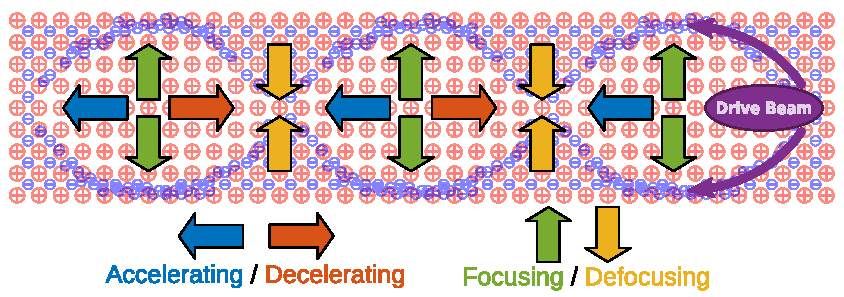
\includegraphics[width=0.85\linewidth,trim={0mm 0mm 0mm 0mm},clip]{figures/PlasmaWakefield}
    \caption{\label{Fig:PWFA:Illust} Illustration of a plasma wakefield accelerating structure with a single electron drive beam. A series of focusing/defocusing and accelerating/deceleratring regions (as seen for an electron witness beam) are produced behind the drive beam.}
\end{figure}

A conceptual illustration of an electron beam driven plasma accelerator is shown in Fig. \ref{Fig:PWFA:Illust}. Several regions of decreasing magnitude of accelerating/decelerating and focusing/defocusing are generated behind the drive beam. By positioning a trailing beam in an optimal phase, such a beam can be both accelerated and focused. The drive beam needs to be shorter than the plasma period for this structure to develop, but multiple short drive beams with a separation of the plasma wave length can resonantly amplify the wakefields.

% ================================================================================================ %
\subsection{The Drive Beam}
\label{Int:BPI:Drive}

The wakefields generated by a charged drive beam are given by the Lorentz force
\begin{equation}
    \vec{W} = \frac{\vec{F}}{q_{b}} = \vec{E} + \vec{v}_{b} \times \vec{B}, \label{EQ:Lorentz}
\end{equation}
where $q_{b}$ is the beam charge and $\vec{v}_{b}$ is the beam velocity. We define the longitudinal coordinate in the frame of the beam along its direction of propagation as
\begin{equation}
    \xi \equiv z - v_{b}t \approx z - ct, \label{EQ:Xi}
\end{equation}
and for the purpose of the following derivations, we use a cylindrical coordinate system $(r, \xi)$. It follows, then, that the longitudinal wakefield is only determined by the longitudinal component of the electric field \dash to the first order \dash such that
\begin{equation}
    W_{\parallel}(r,\xi) = E_{z}(r,\xi). \label{EQ:Wz}
\end{equation}
The transverse wakefield, on the other hand, also depends on the magnetic field such that
\begin{equation}
    W_{\perp}(r,\xi) = E_{r}(r,\xi) - cB_{\theta}(r,\xi), \label{EQ:Wr}
\end{equation}
where we again take the velocity of the beam to be $v_{b} \approx c$.

A charged beam will diverge and lengthen due to space charge, but since the beam is relativistic the effect is of no significance over a few metres of plasma. In the transverse plane, however, the beam is subject to the Lorentz force given by the transverse component of Eq. \ref{EQ:Lorentz}. Taking Maxwell's equations and $B_{\theta} = v_{b}E_{r}/c^{2}$ \cite{schindl:1999}, the strength can be estimated using an infinitely long, uniform beam of density $n_{b}$:
\begin{equation}
    F_{\perp} = q_{b}(E_{r} - v_{b}B_{\theta})
              = q_{b}E_{r}\left(1 - \frac{v_{b}^{2}}{c^{2}}\right)
              = \frac{1}{\gamma^2}q_{b}E_{r}. \label{EQ:DeFocR}
\end{equation}
The implication of this is that for relativistic beams, the transverse dynamics are dominated by emittance and external forces. Dephasing is a potential concern in long plasma sections, and $\Delta L$ over a distance $L$ can be estimated as
\begin{equation}
    \frac{\Delta L}{L} \approx \frac{1}{\gamma^{2}}\frac{\Delta\gamma}{\gamma} \label{EQ:DePhL}
\end{equation}
for two sample particles with energy difference $\Delta\gamma$ \cite{muggli:2017}. For a relativistic beam, this is also not a significant over a fem metres.

% ================================================================================================ %
\subsection{The Transformer Ratio}
\label{Int:BPI:TRat}

The aim of plasma wakefield acceleration is to transfer energy from a drive beam to a witness beam via the plasma. The efficiency of the energy transfer is the ratio of accelerating field amplitude at the position of the witness beam to the decelerating field amplitude within the drive bunch.

Following Ruth \etal \cite{ruth:1985}, let us consider a drive bunch of zero length, with $N_{d}$ particles of individual energy $E_{d}$, and $W_{e}(\xi)$ is the wakefield per unit charge. The energy loss of the bunch in the decelerating field is given by:
\begin{equation}
    \frac{\deriv (N_{d}E_{d})}{\deriv z} = - N_{d}^{2}e^{2}W_{e}(0), \label{EQ:TRat:Drive}
\end{equation}
where $\xi_{d} = 0$ is the position of the drive bunch.

The trailing witness bunch at position $\xi_{w}$, will see the wakefield left by the drive bunch as well as its own wakefield:
\begin{equation}
    \frac{\deriv (N_{w}E_{w})}{\deriv z}
        = - N_{w}^{2}e^{2}W_{e}(0) - N_{d}N_{w}e^{2}W_{e}(\xi_{w}), \label{EQ:TRat:Witness}
\end{equation}
where $N_{w}$ is the number of particles in the witness bunch, and $E_{w}$ is their individual energy.

As required by energy conservation, the total energy of the system cannot increase. It thus follows that
\begin{equation}
    (N_{d}^{2} + N_{w}^{2})W_{e}(0) + N_{d}N_{w}W_{e}(\xi_{w}) \geq 0, \label{EQ:TRat:EConv}
\end{equation}
giving the requirement that the acceleration gradient experienced by a trailing particle satisfies
\begin{equation}
    \frac{\deriv E_{w}}{\deriv z} \leq (2N_{d} - N_{w})e^{2}W_{e}(0). \label{EQ:TRat:Grad}
\end{equation}

Assuming the drive bunch transfers all of its energy to the wakefields, it would stop after a distance
\begin{equation}
    L = \frac{E_{d}}{N_{d}e^{2}W_{e}(0)}. \label{EQ:Trat:LStop}
\end{equation}
The energy a witness beam particle can gain must satisfy
\begin{equation}
    \Delta E_{w} = \frac{\deriv E_{w}}{\deriv z}L
                 \leq E_{d}\left(2-\frac{N_{w}}{N_{d}}\right). \label{EQ:TRat:DeltaE}
\end{equation}

To maximise efficiency in the transfer of energy from the drive beam to the plasma, the beam should have a length $k_{pe}\sigma_{z} \simeq \sqrt{2}$ \cite{lu:2005,lee:2000}. Its transverse size should also stay within $k_{pe}\sigma_{r} \lesssim 1$ as wider beams will cause filamentation instabilities \cite{allen:2012,sentoku:2003}.

The maximum energy gain approaches twice the energy of the drive bunch as $N_{w} \to 0$. In a wakefield accelerator we define the maximum accelerating field \textit{behind} the drive bunch where the witness beam is position, to the maximum decelerating field \textit{within} the drive bunch as the \textit{transformer ratio} \cite{muggli:2017}
\begin{equation}
    R = \frac{E_{+}}{E_{-}}. \label{EQ:TRat}
\end{equation}
While the maximum transformer ratio is $2$, larger values can be achieved by for instance bunch ramping \cite{bane:1985} or by a train of bunches \cite{jing:2006}.

% ================================================================================================ %
\subsection{The Linear Plasma Regime}
\label{Int:BPI:Lin}

When the charge density of the beam is smaller than that of the plasma, $n_{b} \ll n_{pe}$, the system is in the \textit{linear regime}. The linear regime is not of much interest for accelerator applications as it does not utilise the full potential of the plasma for generating strong wakefields, and the transverse and longitudinal fields have continuous variations. These variations will strongly affect the energy spread and emittance of the witness beam. However, this regime is interesting from a theoretical perspective because it is well described analytically \cite{muggli:2017}.

A linear theory for plasma accelerators can be derived using a cold, non-relativistic fluid model of the plasma. The response of the cold plasma can be found from the linearised equations of motion and continuity, and the Maxwell equations. (For examples of linearisation, see \cite{pecseli:2012,chen:1974}.) The equations of motion and continuity are linearised assuming the perturbed plasma density, $n_{1}$, is much smaller than the unperturbed density, $n_{0} = n_{pe}$ \cite{chen:1987}. By further combining the fluid equation and the Poisson equation \cite{katsouleas:1987}, a wave equation for for the plasma density perturbation by the beam can be derived \cite{chen:1987,muggli:2017}:
\begin{equation}
    \frac{\partial^{2}}{\partial\xi^{2}}n_{1} + k_{pe}^{2}n_{1} = \frac{q_{b}}{e}k_{pe}^{2}n_{b}, \label{EQ:BeamPlasmaWF}
\end{equation}
where we still assume $n_{b} \ll n_{pe}$.

The solution to Eq. \ref{EQ:BeamPlasmaWF} in the longitudinal dimension is the Green’s function for a harmonic oscillator in one dimension \cite{katsouleas:1987}, and the radial dependency can be calculated from two-dimensional theory for different radial profiles \cite{chen:1987}. For a beam that has a Gaussian profile in both dimensions, the wakefields are
\begin{align}
    W_{\parallel}(r,\xi) &= \frac{e}{\epsilon_{0}}
        \int_{-\infty}^{\xi} n_{b\parallel}(\xi^{\prime}) \cos\left[k_{pe}(\xi-\xi^{\prime})\right] \,\deriv\xi^{\prime} \,\cdot\, R(r) \label{EQ:WzFull} \\
    W_{\perp}(r,\xi) &= \frac{e}{\epsilon_{0}k_{pe}}
        \int_{-\infty}^{\xi} n_{b\parallel}(\xi^{\prime}) \sin\left[k_{pe}(\xi-\xi^{\prime})\right] \,\deriv\xi^{\prime} \,\cdot\, \frac{\mathrm{d}}{\mathrm{d}r}R(r), \label{EQ:WrFull}
\end{align}
where the transverse dependency $R(r)$ is
\begin{align}
    R(r) &= k_{pe}^{2} \int_{0}^{r} n_{b\perp}(r^{\prime}) I_{0}(k_{pe}r^{\prime})
           K_{0}(k_{pe}r) \,r^{\prime}\,\deriv r^{\prime} \nonumber \\
         &+ k_{pe}^{2} \int_{r}^{\infty} n_{b\perp}(r^{\prime}) I_{0}(k_{pe}r)
           K_{0}(k_{pe}r^{\prime}) \,r^{\prime}\,\deriv r^{\prime}. \label{EQ:WFRadial}
\end{align}
Here $I_{0}$ and $K_{0}$ are the zeroth-order modified Bessel functions of the first and second kind, respectively \cite{chen:1987,muggli:2017}.

\begin{figure}[hbt]
    \centering
    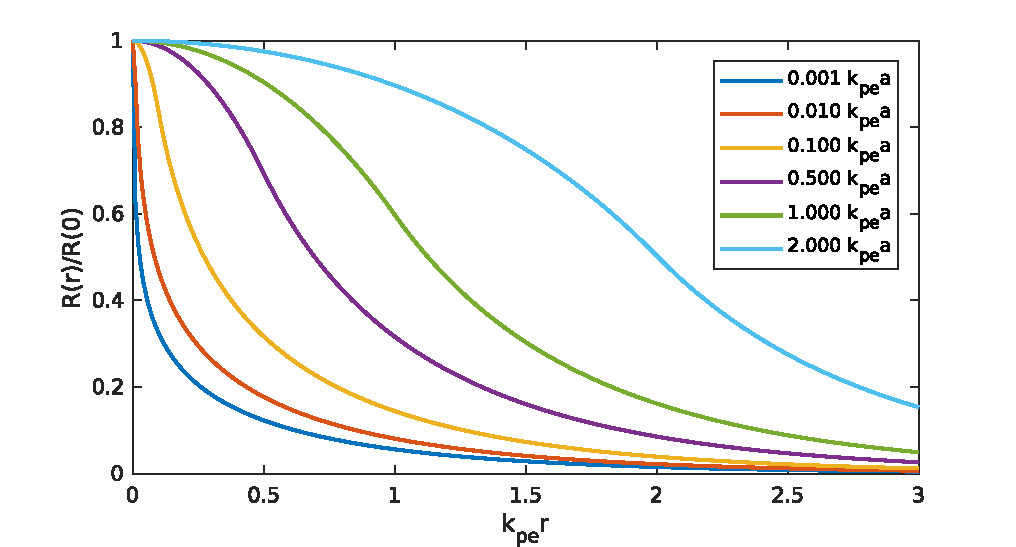
\includegraphics[width=0.8125\linewidth,trim={0mm 0mm 0mm 0mm},clip]{figures/RepKatsouleas1987}
    \caption{\label{Fig:BPI:Kat87} The radial function $R(r)$ for a range of uniform beams cut off at a radius $a$ up to twice the plasma skin depth $k_{pe}^{-1}$. The plot is reproduced from Katsouleas \etal \cite{katsouleas:1987}.}
\end{figure}

As can be seen from Figure \ref{Fig:BPI:Kat87}, the longitudinal wakefield is at its maximum on-axis. For very wide beams, $\sigma_{r} \gg k_{pe}$, we converge at the one-dimensional result. For very narrow beams, $\sigma_{r} \ll k_{pe}$, the maximum decreases rapidly with radius causing different parts of the witness beam at different radii to see different accelerating fields. The cosine component of Eq. \ref{EQ:WzFull} also implies longitudinal variations of the accelerating field. Combined, these produce a large energy spread for the accelerating beam. Additionally, the sinusoidally varying focusing field from Eq. \ref{EQ:WrFull} produces emittance growth \cite{muggli:2017,katsouleas:1987}.

% ================================================================================================ %
\subsection{The Non-Linear Plasma Regime}
\label{Int:BPI:NLin}

When the beam density $n_{b} > n_{pe}$, the system enters the non-linear regime, and becomes highly non-linear when $n_{b} \gg n_{pe}$ \dash often referred to as the \textit{blowout} regime. Using this regime for plasma wakefield acceleration was proposed by Rosenzweig \etal in 1991 \cite{rosenzweig:1991}. In this regime the plasma electrons are expelled entirely from the region around the axis to form a region populated by only plasma ions. As the ions are practically stationary on the time scale of the plasma electrons, they form a uniform column of positive charge. The electrons displaced by the space charge of the drive beam are pulled back on axis by the ions in the form a thin sheath with the shape of a bubble. Hence, this regime is also sometimes referred to as the \textit{bubble regime}. The large transverse forces produced by the drive beam in this regime, followed by the strong restoring force of the ion channel, produces a large density spike behind the formed bubble \cite{dawson:1959,rosenzweig:1991}.

[Reproduce plots in figure 2 of Rosenzweig 1991 from QuickPIC data and insert here.]

The radial wakefield, $W_{r}$, produces linear focusing, while the accelerating wakefield, $W_{\xi}$, is uniform within the bubble. In other words: while the focusing prevents emittance growth, the accelerating gradient of the witness bunch, being independent of radial position for a range of positions, avoids large energy spreads \dash both disadvantages with the linear regime.

Unlike in the linear case, there is no full theory describing the non-linear case. However, a non-linear kinetic theory has been developed by Lu \etal that is valid under certain assumed conditions \cite{lu:2006a,lu:2006}.

% ================================================================================================ %
\subsection{Beam Loading}
\label{Int:BPI:BLoad}

A challenge with both the linear and the non-linear regime is the longitudinally varying accelerating field, producing energy spread in the accelerated bunch. Ideally, the accelerating field should be uniform in the region occupied by the witness bunch. As the witness bunch generates its own wakefield, these fields are combined with those from the drive bunch. It follows, then, that the properties of the witness bunch can both worsen and improve the flatness of the field.

[Add beam loading plot, or combine with plot from previous subsection]

In the linear case, the challenge is to create a uniform accelerating field in both the transverse and longitudinal direction. The non-uniformity challenges have been outlined, and solutions proposed, by Van der Meer \cite{van_der_meer:1985} as well as Katsouleas \etal \cite{katsouleas:1987} in the 1980s. The latter suggesting triangular and trapezoidal witness bunches in order to exactly cancel the variations in the field within the bunch.

In the non-linear case, the radial accelerating field variation vanishes, provided witness bunch transverse size is within about $2\sigma_{r}$ of the drive bunch \cite{rosenzweig:1991}. The longitudinal variation, however, remains.

A short bunch with respect to the accelerating phase of the wakefield, $L \leq \lambda_{pe}/4$, will affect the shape of the plasma electron sheath, but still allow them to return to the axis while decreasing their transverse momentum. If the total momentum reaches zero, the witness beam has extracted all the energy of the accelerating field \cite{lu:2006a,lu:2006}. This is generally not achievable, but as outlined by Tzoufras \etal \cite{tzoufras:2009}, a trapezoidal witness bunch, with a density maximum at its head, can theoretically both flatten the field and achieve a high transformer ratio. They further show that a flat top bunch is similarly efficient, and Gaussian bunches also have comparable properties \dash all being sensitive to fine tuning of position within the bubble, as well as its spot size.

Tzoufras \etal provides a solution for the energy absorbed per unit length for an ideal trapezoidal bunch. stating that
\begin{equation}
    Q_{tr}E_{t} = \frac{\pi R_{b}^{4}}{16}, \label{EQ:Trapez}
\end{equation}
where $Q_{tr}$ is the total charge of the trapezoidal bunch, $E_{t}$ is the longitudinal field at the head of the bunch, and $R_{b}$ is the radius of the bubble. It immediately follows that at optimal beam loading, there is a trade-off between charge and the accelerating gradient and thus energy gain \cite{tzoufras:2009}.

% ================================================================================================ %
\subsection{Beam Matching}
\label{Int:BPI:Match}

In the non-linear case, where an ion column is formed, the focusing force it produces will cause a pinching effect on the beam. While the beam itself, assuming $\emitN > 0$, will try to expand, there exists a beam radius where the focusing force and the beam's tendency to expand are in equilibrium. For a highly relativistic beam, $\gammar \gg 1$, the equilibrium radius is given by \cite{krall:1995}
\begin{equation}
    \sigma_{r,\mathrm{eq}} = \left( 8 \frac{\emitN^2}{\gammar} \frac{c^2}{\omega_{p}^2} \right)^{1/4}. \label{EQ:BMatch}
\end{equation}

This follows from the general envelope equation \cite{lee:1976} under the assumption that: the beam enters the plasma at focus (i.e. $\deriv\sigma_{r}/\deriv z = 0$), does not diverge significantly from a Gaussian transverse density profile, and that the focusing force is linear \cite{krall:1995}.

\begin{figure}[hbt]
    \centering
    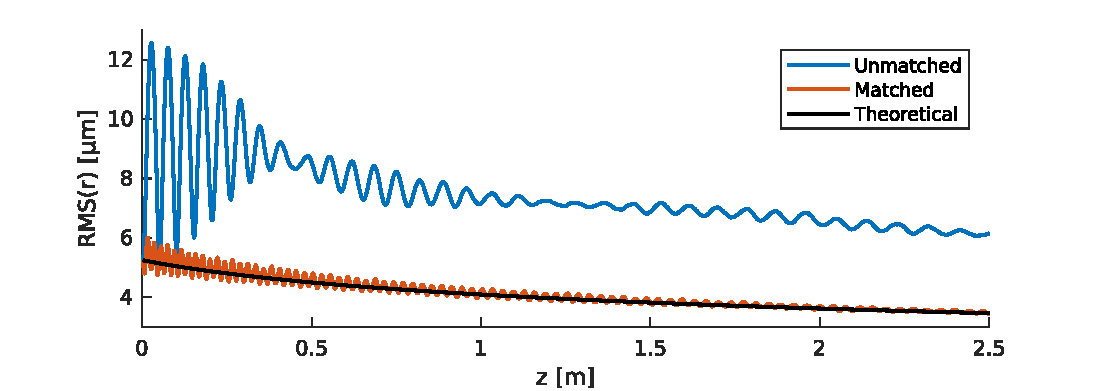
\includegraphics[width=0.875\linewidth,trim={0mm 0mm 0mm 0mm},clip]{figures/BeamMatching}
    \caption{\label{Fig:BPI:Match} The evolution of the transverse RMS size of an initially matched electron beam as it accelerates through a plasma. The tail of the beam, in red, remains in a region where it is matched, while the head of the beam, in blue, does not. The black line corresponds to the theoretical spot size of the beam at nominal plasma density. Based on simulation data from Publication \ref{Pub:BL17}.}
\end{figure}

The simulation in Figure \ref{Fig:BPI:Match} shows the evolution of the transverse RMS size of an electron beam as it travels through a plasma. The beam has a normalised emittance of $2\unit{\mu m}$, and is initially matched to a plasma density of $7\nexp{14}\unit{cm}^{-3}$ with a $\sigma_{r} = 5.24\unit{\mu m}$. The tail of the beam, in red, is in the plasma bubble and thus sees an ion density equal to the plasma density. The head of the beam, in blue, where the bubble is forming, sees a lower density. It is thus not matched, and instead oscillates around an equilibrium point at a larger radius. The black line is the predicted $\sigma_{r}$ given by Eq. \ref{EQ:BMatch} at initial plasma density, and beam energy as a function of $z$ as the beam is accelerated \cite{berglyd_olsen:2018}.

% ================================================================================================ %
\subsection{Multiple Drive Bunches}
\label{Int:BPI:Multi}

As discussed above, higher transformer ratios can be achieved with multiple drive bunches with a $\lambda_{pe}$ separation. This happens because such a train of bunches will resonantly drive increasing wakefields.

As outlined by Kallos \etal \cite{kallos:2007}, if the bunches are longitudinally square, the wakefields scale linearly with the number of bunches. The shape is of less importance if the bunch length is much less than $\lambda_{pe}$. However, this does not result in high efficiency as every trailing bunch will see the decelerating field of the earlier bunches. Efficiency is instead increased when each bunch experience a similar wake field.

This effect can be mitigated in two ways that will in turn maximise transformer ratio. The first option, named \textit{Ramped Bunch Train}, is to position the bunches with a $1.5\cdot\lambda_{pe}$ separation, such that each bunch is in the accelerating phase, while at the same time ramp their charge such that the wakefield inside each bunch matches the decelerating field from the first bunch. This scheme has been demonstrated experimentally by Jing \etal \cite{jing:2006,jing:2007}.

The second method described by Kallos \etal, called \textit{Phased Bunch Train}, proposes using short, $k_{pe}l_{z} \ll 1$, equally charged bunches placed in a specific decelerating phase. The bunch separation needs to be tuned so that the fields inside each bunch matches that of the first bunch. The phase shift $\theta_{M}$ for the $M$-th bunch is described by Ruth \etal \cite{ruth:1985}:
\begin{equation}
    \theta_{M} = \sum^{M}_{n=2}\tan^{-1}\left(\frac{1}{\sqrt{n-2}}\right),\quad M \geq 2. \label{EQ:TrainPhase}
\end{equation}
This yields a maximum energy gain
\begin{equation}
    \Delta E_{w} = E_{d,1}\left(2\sqrt{M}-\frac{N_{w}}{N_{d,1}}\right), \label{EQ:TrainPhaseMaxE}
\end{equation}
where $N_{d,1}$ is the first of $M$ drive bunches. Compared to Eq. \ref{EQ:TRat:DeltaE} this is an improvement, although not linearly increasing with the number of bunches \cite{ruth:1985}.

% ================================================================================================ %
\section{Using a Proton Drive Beam}
\label{Int:DBeam}

So far the theory presented has focused on short electron bunches as drivers for plasma wakefield acceleration. Electron bunches used in such experiments have a low total energy and thus a limited propagation length in the plasma, as can be estimated using Eq. \ref{EQ:Trat:LStop}.

One experiment, at the Stanford Linear Accelerator Center (SLAC) \cite{blumenfeld:2007}, achieved up to a doubling of energy of electrons with a $42\unit{GeV}$ driver with $1.8\nexp{10}$ particles, corresponding to a total beam energy of $120\unit{J}$. The propagation length of such a beam is on the order of a metre, and the experiment used an $85\unit{cm}$ lithium plasma cell to achieve the energy doubling, with a gradient of up to $52\unit{GeV}$. Such short accelerator segments are suitable for multi staged accelerators, but they require multiple high energy electron beams. 

% ================================================================================================ %
\subsection{Protons vs. Electrons as Drive Beam}
\label{Int:DBeam:PDPWFA}

AS ultra-high energy electron bunches are not readily available, it is tempting to suggest using protons as drivers instead. The much higher mass carries orders of magnitude more energy at relatively low gamma values. This effectively eliminates the problem with short propagation lengths in plasma as it scales linearly with the beam energy; see Eq. \ref{EQ:Trat:LStop}.

[Table of proton beam energies]

Add: challenge of producing short bunches.

Cite \cite{adli:2016a,adli:2016b}.

The problem with $\gg\lambda_{pe}$ proton bunches can be solved by exploiting one of several instabilities that can occur when a long bunch propagates through plasma.
% ================================================================================================ %
\subsection{The Self-modulation Instability}
\label{Int:DBeam:SMI}

A long beam with respect to the plasma wavelength will generate a density wave driven by its own head. This is true for both laser beams \cite{esarey:1994} and particle beams \cite{kumar:2010}, and they are caused by the same underlying physics. For a laser beam, this produces alternating regions of focusing and diffraction. For a particle beam, the wakefields generated within the beam acts back on itself, breaking it up into short micro bunches with a surrounding, defocused halo.

In the 1980s, this self-modulating effect was taken advantage of in LWFA experiments as only long laser pulses were available. Advances in ultra short laser technology later removed the dependence of this effect \cite{pukhov:2002}, however for proton drive beams this is still an issue. For instance, the SPS proton beam used by AWAKE is orders of magnitude longer than the plasma wavelength needed for the experiment.

The self-modulation instability (SMI), is one of several instabilities affecting long beams in plasma.

% To add: Phase velocity of SMI WF. Two-stream and hosing.

In electron beam \cite{muggli:2014}.

% ================================================================================================ %
